\documentclass[hidelinks,pdftex,phd]{pittetd} 
\overfullrule=0pt
%CHAPTER NUMBERING
%1) default = No specification needed
        %Chapters with numbers (1.0, 2.0, etc.) 
        %sections with numbers and sub-numbers (1.1, 1.2, 2.1, 2.2, etc.) 
        %subsections with numbers and sub-numbers (an additional sub-number) (1.1.1, 1.1.2, 2.1.1, 2.1.2, etc)
        %subsubsections with numbers and sub-numbers (two additional sub-numbers) (1.1.1.1, 1.1.1.2, 2.1.1.1, 2.1.1.2, etc.)
%2)'sectionletters'= Changes numbering format
        %Chapters with Roman numerals (I, II, etc.) 
        %sections with letters (A, B) 
        %subsections with numbers (1, 2)
        %subsubsections with lowercase letters (a, b)

%SPECIAL OPTIONS
%VERSION
%1)'final' = Changes all "format warnings" into errors (Final version of the document       

%%%%%%%%%%%%%%%%%%%%%%%%%%%%%%%%%%%%%%%%%%%%%%%%%%%%%%%%%%%%%%%%%%%%%%%%%%%%%%%%%%%%%%%%%%%%%%%%%%%
% Default includes
%%%%%%%%%%%%%%%%%%%%%%%%%%%%%%%%%%%%%%%%%%%%%%%%%%%%%%%%%%%%%%%%%%%%%%%%%%%%%%%%%%%%%%%%%%%%%%%%%%%
\usepackage{graphicx}
\usepackage{indentfirst}
\usepackage{amsmath,amsthm}
\usepackage{pdflscape}
\hypersetup{hidelinks}
\patch{amsmath}
\patch{amsthm}
\makeatletter
\renewcommand{\@biblabel}[1]{[#1]\hfill}
\makeatother
\makeatletter
\def\@hangfrom#1{\setbox\@tempboxa\hbox{{#1}}%
      \hangindent 0pt%\wd\@tempboxa
      \noindent\box\@tempboxa}
\makeatother

%%%%%%%%%%%%%%%%%%%%%%%%%%%%%%%%%%%%%%%%%%%%%%%%%%%%%%%%%%%%%%%%%%%%%%%%%%%%%%%%%%%%%%%%%%%%%%%%%%%
% Additional includes
%%%%%%%%%%%%%%%%%%%%%%%%%%%%%%%%%%%%%%%%%%%%%%%%%%%%%%%%%%%%%%%%%%%%%%%%%%%%%%%%%%%%%%%%%%%%%%%%%%%
% Chapter 2
\usepackage{multirow}
% Chapter 3
\usepackage{physics}
\usepackage[version=4]{mhchem}
\usepackage{siunitx}
\newcommand{\angstrom}{\mbox{\normalfont\AA}}
\sisetup{load-configurations = abbreviations}
\usepackage{tablefootnote}
\usepackage{booktabs}
\usepackage{threeparttable}
% Appendix 2
\usepackage{subcaption}
\usepackage[ruled, vlined, linesnumbered, commentsnumbered]{algorithm2e}
\usepackage{tikz}
\newcommand*\circled[1]{\tikz[baseline=(char.base)]{
  \node[shape=circle,draw,fill=black,text=white,font=\bf,inner sep=0.5pt] (char)
  {\scriptsize#1};
}}

\newcommand*\circledwhite[1]{\tikz[baseline=(char.base)]{
  \node[shape=circle,draw,fill=white,text=black,font=\bf,inner sep=0.5pt] (char)
  {\scriptsize#1};
}}
%%%%%%%%%%%%%%%%%%%%%%%%%%%%%%%%%%%%%%%%%%%%%%%%%%%%%%%%%%%%%%%%%%%%%%%%%%%%%%%%%%%%%%%%%%%%%%%%%%%
% Change Figure and Table Numeration
%%%%%%%%%%%%%%%%%%%%%%%%%%%%%%%%%%%%%%%%%%%%%%%%%%%%%%%%%%%%%%%%%%%%%%%%%%%%%%%%%%%%%%%%%%%%%%%%%%%
%\chapterfloats %Uncomment this to get figures and tables numbered within chapters.

%%%%%%%%%%%%%%%%%%%%%%%%%%%%%%%%%%%%%%%%%%%%%%%%%%%%%%%%%%%%%%%%%%%%%%%%%%%%%%%%%%%%%%%%%%%%%%%%%%%
\title[Theoretical Treatment of Weakly Bound Fermions to Atoms, Molecules, and Clusters]{Theoretical Treatment of Weakly Bound Fermions to Atoms, Molecules, and Clusters}
\author{Shiv Upadhyay}
\degree{Master of Science, Duquesne University, 2017\\Bachelor's of Arts, Washington and Jefferson College, 2015}
\school{Dietrich School of Arts and Sciences}
\date{\today}
%\year{2022}
\setyear{2022}
\keywords{hail-to-pitt, pittetd, theses, format}
\subject{Dissertation}
%%%%%%%%%%%%%%%%%%%%%%%%%%%%%%%%%%%%%%%%%%%%%%%%%%%%%%%%%%%%%%%%%%%%%%%%%%%%%%%%%%%%%%%%%%%%%%%%%%%
\committeemember{Kenneth D. Jordan, Richard King Mellon Professor and Distinguished Professor of
Computational Chemistry, Department of Chemistry}
\committeemember{Geoffrey Hutchison,  Associate Professor, Department of Chemistry}
\committeemember{Peng Liu, Associate Professor, Department of Chemistry}
\committeemember{David Yaron, Professor, Department of Chemistry, Carnegie Mellon University}
%%%%%%%%%%%%%%%%%%%%%%%%%%%%%%%%%%%%%%%%%%%%%%%%%%%%%%%%%%%%%%%%%%%%%%%%%%%%%%%%%%%%%%%%%%%%%%%%%%%
\raggedbottom



\begin{document}

\maketitle
%%%%%%%%%%%%%%%%%%%%%%%%%%%%%%%%%%%%%%%%%%%%%%%%%%%%%%%%%%%%%%%%%%%%%%%%%%%%%%%%%%%%%%%%%%%%%%%%%%%
\committeemember{Kenneth D. Jordan, Advisor Departmental Affiliation}
\committeemember{Second member's name, Departmental Affiliation}
\committeemember{Third member's name, Departmental Affiliation}
\school{Department of Mathematics}
\makecommittee
%%%%%%%%%%%%%%%%%%%%%%%%%%%%%%%%%%%%%%%%%%%%%%%%%%%%%%%%%%%%%%%%%%%%%%%%%%%%%%%%%%%%%%%%%%%%%%%%%%%
\copyrightpage                     
%%%%%%%%%%%%%%%%%%%%%%%%%%%%%%%%%%%%%%%%%%%%%%%%%%%%%%%%%%%%%%%%%%%%%%%%%%%%%%%%%%%%%%%%%%%%%%%%%%%
\begin{abstract}
The abstract of the document.
This document is a sample file for the creation of ETD's at Pitt through \LaTeX.
\end{abstract}
%%%%%%%%%%%%%%%%%%%%%%%%%%%%%%%%%%%%%%%%%%%%%%%%%%%%%%%%%%%%%%%%%%%%%%%%%%%%%%%%%%%%%%%%%%%%%%%%%%%

\tableofcontents
\listoftables                      
\listoffigures                
%%%%%%%%%%%%%%%%%%%%%%%%%%%%%%%%%%%%%%%%%%%%%%%%%%%%%%%%%%%%%%%%%%%%%%%%%%%%%%%%%%%%%%%%%%%%%%%%%%%
\phantomsection
\preface
This is the text of the preface, with acknowledgments, dedication, etc. 
%%%%%%%%%%%%%%%%%%%%%%%%%%%%%%%%%%%%%%%%%%%%%%%%%%%%%%%%%%%%%%%%%%%%%%%%%%%%%%%%%%%%%%%%%%%%%%%%%%%
%
% MAIN DOCUMENT
%
%%%%%%%%%%%%%%%%%%%%%%%%%%%%%%%%%%%%%%%%%%%%%%%%%%%%%%%%%%%%%%%%%%%%%%%%%%%%%%%%%%%%%%%%%%%%%%%%%%%

\chapter{Introduction}

Chemistry involves the study of molecules and materials constructed from nuclei and electrons.
The theoretical description of a chemical system requires a consideration of the size of the system and of the target properties.
An ideal computational chemistry theoretical model would reproduce experimental observables in a computationally tractable amount of time.
In the following sections, Nonvalence anions and the related nonvalence positronic bound states are introduced along with the target properties of interest followed by a discussion of the computational chemistry methods used to describe these systems.

%%%%%%%%%%%%%%%%%%%%%%%%%%%%%%%%%%%%%%%%%%%%%%%%%%%%%%%%%%%%%%%%%%%%%%%%%%%%%%%%%%%%%%%%%%%%%%%%%%%
\section{Chemical Systems}
%%%%%%%%%%%%%%%%%%%%%%%%%%%%%%%%%%%%%%%%%%%%%%%%%%%%%%%%%%%%%%%%%%%%%%%%%%%%%%%%%%%%%%%%%%%%%%%%%%%
% Nonvalence Anions
\subsection{Nonvalence Anions}

Nonvalence anions are formed when a molecule weakly captures an electron in an extremely diffuse orbital.
It is helpful to further differentiate nonvalence anions due to the dominant mechanism of binding into nonvalence electrostatically bound anions (NVEBs) and nonvalence correlation bound anions (NVCBs).
Nonvalence electrostatically bound anions bind an electron using a permanent electrostatic moment.
For example, an electron can be captured by a molecule or molecular cluster with a sufficiently strong dipole moment, creating a nonvalence electrostatically bound anion also called a dipole bound anion (DBA).
Nonvalence correlation bound anions require electron correlation effects to account for the binding of the electron.
This is not to say that the neutral system giving rise to a NVCB lacks any permanent electric moments, but rather, that the uncorrelated description of a system containing these permanent moments will not bind the electron.
%The discussion below includes a more detailed description of these systems along with paradigmatic examples.

\subsubsection{Nonvalence Electrostatically Bound Anions}

Dipole-bound anions (DBAs) are formed when a molecule with sufficiently large dipole moments (1.625 D in the Born-Oppenheimer approximation) capture an electron in a diffuse, nonvalence orbital.\cite{Jordan_Luken_JCP_1976,Gutowski_Jordan_PRA_1996,Barnett_JCP_1988,Fermi_Teller_PhysRev_1947,Turner_Anderson_PhysRev_1968,Crawford_ProcPhysSoc_1967,Garrett_CPL_1970,Garrett_PRA_1971,Lykke_PRL_1984,Desfrancois_Schermann_PRL_1994,Simons_JPCA_2008,Jordan_Wang_Ann_Rev_2003}.
Initially, one may be tempted to think that electron correlation would not play a significant role in such systems given the diffuse nature of the excess electron.
However the excess electron is bound far from the valence electrons, there is a dispersion interaction between the excess electron and the neutral molecule.\cite{Gutowski97,Gutowski98}
However, considering the simplified expression for London dispersion it can be seen that the dispersion interaction is dependent on the polarizability of the two interacting entities.\cite{London1937}
\begin{equation}
	E_{\mathrm{Disp}} = -\left(\frac{3h}{2R^6}\right) \left(\alpha_i \alpha_j \right) \left(\frac{\nu_k \nu_j}{\nu_k + \nu_j} \right)
\end{equation}
where $\alpha$ is the static polarizability, $\nu$ is the ionization potential, and $R$ is the separation distance.
The diffuse electron is spread over a large volume, and therefore has a large polarizability leading to a large dispersion interaction.

\begin{figure}{r}
    \centering
	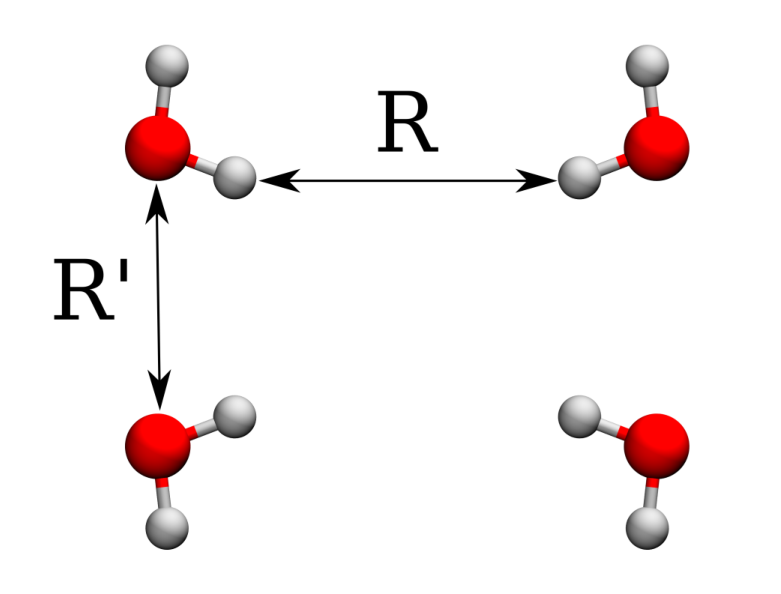
\includegraphics[width=0.9\textwidth,keepaspectratio]{Images/chapter1/h2o4_labeled.eps}
	\caption{A model \ce{(H2O)4} system. The separation between the dimers $R$ is variable, but the separation of two waters within each dimer $r=\SI{2.77514}{\angstrom}$ is fixed.}
	\label{fig:h2o4}
\end{figure}
Nonvalence correlation bound anions are similar to DBAs, but the leading contribution to the binding energy comes from electronic correlation.
Often this means NVCB anions do not posses a dipole moment.
For DBAs, the Hartree-Fock can bind an electron for molecules with dipole moments above the critical threshold, although the electron would be considerably underbound.
For NVCB anions, it has been shown that the HF solution is qualitatively incorrect.
Rather than binding the electron, the HF solution collapses onto the continuum yielding a wavefunction for the neutral plus an excess electron in a continuum orbital.
When this occurs, methods that build upon the HF result such as single reference perturbation theory, or even coupled cluster methods, will also fail to bind the excess electron.
A simple example of this is a model water tetramer cluster that has been studied previously in our group.\cite{Voora2017}
This model system can be seen in fig.~\ref{fig:h2o4}.
This system has no dipole moment, and the electron is bound by electrostatics and correlation effects.
By increasing the separation between the two pairs of water dimers, one can induce a crossover from a nonvalence electrostatically-bound anion to a nonvalence \textit{correlation-bound} anion.
DBAs can serve as a pathway to valence-bound anions\cite{Hendricks_JCP_1998,Compton_JCP_1996,Desfrancois_JCP_1996,Desfrancois_JPCA_1998}, and nonvalence correlation bound anions can as well. \cite{Voora20142}

\begin{figure}{r}
	\centering
	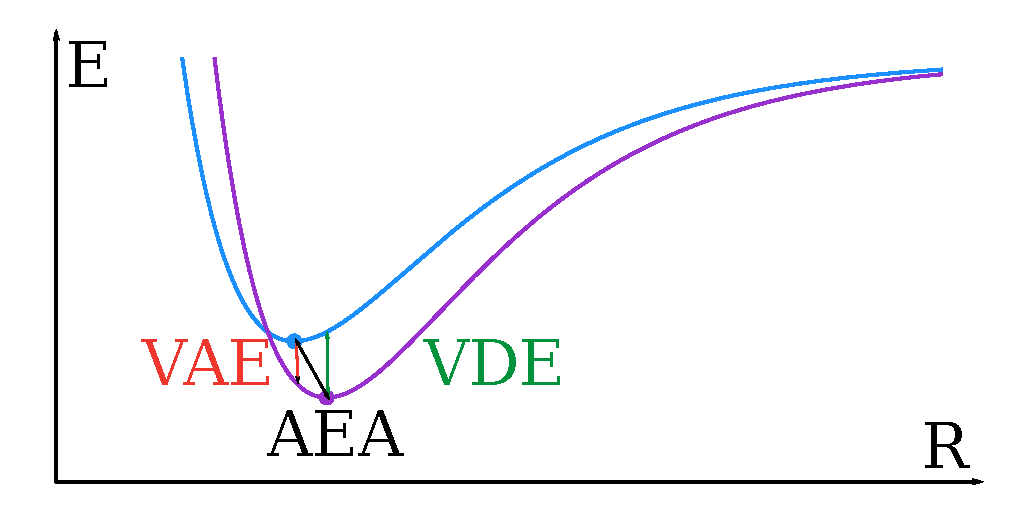
\includegraphics[width=0.9\textwidth,keepaspectratio]{Images/chapter1/morse.eps}
	\caption{Illustrative potential energy curves for a neutral molecule and its corresponding dipole-bound or correlation-bound anion. The energy difference at the neutral geometry is the vertical attachment energy. The energy difference at the anion geometry is the vertical detachment energy. The energy difference between the two respective minima is the \textbf{adiabatic electron affinity}.}
	\label{fig:morse}
\end{figure}

Fig.~\ref{fig:morse} shows illustrative potential energy curves for a hypothetical bound anion.
The coordinate ($R$) represents a collective variable which captures the change in geometry ($\delta R$) that the neutral molecule undergoes upon capturing an electron.
The change in energy associated with binding the electron and the subsequent change in geometry is termed the adiabatic electron affinity.
The change in energy associated only with binding the electron may occur at either the neutral or anionic geometry and is termed the vertical electron affinity and vertical detachment energy respectively.
The extremely diffuse nature of the excess electron in DBAs and NVCB anions often results in a very minor change in geometry.
In the limit of zero change in geometry ($\delta R \rightarrow 0$), the adiabatic electron affinity, vertical electron affinity, vertical detachment energy are equal.
Therefore, for DBAs it is sufficient to calculate only one of these energies.
In practice, and in this work, it is easiest to calculate the vertical electron affinity as this only requires the ground state neutral geometry.
%The dipole-bound anion may not be the lowest energy anion which could lead to difficulties as optimizing an excited state geometry can be a numerically difficult procedure.
%For example, if one is optimizing a geometry for a CIS excited state, one must ensure that the same state is being located at all points of an optimization.
%This could happen because the initial
The magnitude by which the electron is bound is also referred to as the electron binding energy (EBE).
The sign convention adopted is that a positive electron binding energy indicates that the the electron is bound.

%%%%%%%%%%%%%%%%%%%%%%%%%%%%%%%%%%%%%%%%%%%%%%%%%%%%%%%%%%%%%%%%%%%%%%%%%%%%%%%%%%%%%%%%%%%%%%%%%%%
% Positron bound states
\subsection{Positron bound states}
Since the theoretical prediction\citehere and subsequent experimental observation\citehere of positrons, the exotic antimatter has seen use in a variety of fields such as positron emission tomography in the medical field or in defect characterization in condensed matter physics.\citehere
Modern applications have also included the formation of antihydrogen as a test of fundamental physics regarding violations of charge, parity, and time-reversal symmetries.\citehere

In chemistry, one is interested in the behavior of matter.
It may seem that the study of antimatter is of little interest to chemistry, however through electron-positron interactions serve as an experimental probe to understand the electronic and vibronic structure of molecules.

In order to understand how positrons yield insight into the behavior of molecules, it helps to consider the interaction of a low energy positron with an idealized molecule.
The simplest picture of this process would imply that the positron and electron annihilation rate would be proportional to the number of electrons present.\citehere %surko rev mod
Interestingly, the observed rate of annihilation is orders of magnitude greater for most molecules.\citehere %surko rev mod
The major causes of this increased annihilation rate is the formation of positron-molecule bound states and positron-molecule temporary states (vibrational Feschbach resonances).\citehere
Since the processes are molecule dependent, the experimental characterization of positron annihilation allows one to characterize different molecules.
This also explains the motivation to computationally study positron bound states.
The diffuse positronic states are diffuse analogues to nonvalence anions with direct connection to experiment.

%%%%%%%%%%%%%%%%%%%%%%%%%%%%%%%%%%%%%%%%%%%%%%%%%%%%%%%%%%%%%%%%%%%%%%%%%%%%%%%%%%%%%%%%%%%%%%%%%%%

\section{Theoretical Methods}
%%%%%%%%%%%%%%%%%%%%%%%%%%%%%%%%%%%%%%%%%%%%%%%%%%%%%%%%%%%%%%%%%%%%%%%%%%%%%%%%%%%%%%%%%%%%%%%%%%%
% Molecular quantum mechanics
\subsection{Molecular Quantum mechanics}
\subsubsection{Schrodinger's Equation}
\subsubsection{Born Oppenheimer Approximation}

%%%%%%%%%%%%%%%%%%%%%%%%%%%%%%%%%%%%%%%%%%%%%%%%%%%%%%%%%%%%%%%%%%%%%%%%%%%%%%%%%%%%%%%%%%%%%%%%%%%
% Many Body Methods
% Mean Field Methods
\subsection{Basis}
Invoking the \gls{boa}, allows us to define a basis for the electronic degrees of freedom.
Since the goal is to represent the electron density that is expected to be localized around the nuclei, a natural basis for representing this density is a set of \glspl{ao} centered at the nuclei.
For computational reasons, gaussian orbitals are used to represent \glspl{mo},
\begin{equation}
\psi_{\textrm{MO}} = \sum_{i} \Phi_{\textrm{AO}} = \sum_{i} N(L, \alpha) Y_{lm}(\theta, \phi) e^{-\alpha |r - R_A|^2},
\end{equation}
where $r_A$ is the location of the atomic center where this gaussian orbital is centered, $Y_{lm}(\theta, \phi)$ is a spherical harmonic, and $N(L, \alpha)$ is a normalization constant.
This approach is also called the \glsxtrlong{lcao}.

As a simple example for a two electron problem, we write the wave function using the \gls{lcao} approach,
\begin{equation}
\Psi = \phi_{MO1}(r_1) \phi_{MO2}(r_2).
\label{eq:hartreeproduct}
\end{equation}
However, since electrons are fermions any wave function ansatz must be antisymmetric.
The ansatz in eq.~\ref{eq:hartreeproduct}, also known as the Hartree product, is not antisymmetric,
\begin{equation}
\Psi(1,2) = \phi_{MO1}(r_1) \phi_{MO2}(r_2) \neq -\phi_{MO1}(r_2) \phi_{MO2}(r_1) = -\Psi(2,1).
\end{equation}
This can be remedied by writing the ansatz wave function as, 
\begin{equation}
\Psi = \phi_{MO1}(r_1) \phi_{MO2}(r_2) - \phi_{MO1}(r_2) \phi_{MO2}(r_1),
\label{eq:2pslaterdet}
\end{equation}
which can be easily verified to be antisymmetric by interchanging the two particles.
The expansion in eq.~\ref{eq:2pslaterdet} is the expansion of a determinant of a 2$\times$2 matrix.
The generalization of the ansatz for N electrons is a \gls{sd},
\begin{eqnarray}
	\Psi(r_1,r_2,...,r_N) &=& \frac{1}{\sqrt{N!}} 
		\left|
			\begin{array}{cccc}
				\phi_1(r_1) & \phi_2(r_1) & \ldots & \phi_N(r_1) \\
				\phi_1(r_2) & \phi_2(r_2) & \ldots & \phi_N(r_2) \\
				\vdots      & \vdots      &        & \vdots      \\
				\phi_1(r_N) & \phi_2(r_N) & \ldots & \phi_N(r_N) \\
			\end{array}
		\right|.
\end{eqnarray}
\glsxtrfullpl{sd} serve as the many electron wave function basis for our calculations.

\subsection{Mean Field Methods}
The electronic time independent Schrodinger equation is still a many body problem, and due to its multidimensional nature, it does not lend itself to an easy solution.
The common approximation for many body problems in physics is a mean-field approximation.
Mean-field approximations involve mapping an interacting problem onto a noninteracting problem with averaged interactions.
The Hartree-Fock method involves mapping the interacting quantum many-body problem onto a noninteracting problem with each electron interacting with the average potential of the other electrons.
Since the average potential that each electron experiences is dependent on the density of each of the other electrons, the solution to the Hartree-Fock equations must be found iteratively.
This means that the independent particle densities yield averaged interaction potentials that yield new independent particle densities, and this process is repeated.
Eventually, the previous iteration's densities are unchanged in an iteration, a condition termed self-consistency.
Once this condition has been fulfilled, we stop iterating, and we have found the mean-field solution.

\shiv{add hf algo}
The above described Hartree-Fock algorithm for a Slater determinant trial wavefunction is given in listing 1.
The linear algebra machinery makes the Hartree-Fock method amenable to solution on modern computational hardware.

%%%%%%%%%%%%%%%%%%%%%%%%%%%%%%%%%%%%%%%%%%%%%%%%%%%%%%%%%%%%%%%%%%%%%%%%%%%%%%%%%%%%%%%%%%%%%%%%%%%
% Correlation Methods
% TODO edit here
\subsection{Correlated Methods}

\shiv{define correlation}

\subsubsection{Density Functional Theory Methods}
\gls{dft} has seen widespread use since it is an economical, albeit approximate, treatment of electron correlation.\citehere

\gls{dft} in theory is an exact method.
The first Hohenberg-Kohn theorem establishes an exact mapping between the interaction potential and the electron density.\citehere
The second Hohenberg-Kohn theorem shows that a variational principle for the energy as a functional of the density exists.\citehere
While these theorems and extensions for finite temperature, magnetic fields, and other generalizations,\citehere solidify \gls{dft}'s theoretical footing, they do not indicate how one would practically use \gls{dft}.

In practice, the Kohn-Sham equations are used which maps the density-based Schr{\"o}dinger equation problem on to a fictious noninteracting problem with an effective field,
\begin{equation}
(\hat{T} + \hat{V}_{\mathrm{eff}}) \psi(r) = E \psi(r).
\end{equation}
This formulation resembles a \gls{hf} equation where the interaction potential has been replaced by an effective potential.
This allows one to utilize the standard \gls{hf} machinery and incorporate electron correlation at minimal cost.
The form of the effective potential is what is commonly referred to as the \gls{dft} functional.
These functionals are constructed and parameterized as the exact functional is not known.
This means that althought \gls{dft} is an exact theory, in practice it is not \textit{ab initio}.



\subsubsection{Wave Function Based Methods}
Wave function based correlated methods build upon  the uncorrelated \gls{hf} reference and attempt to reincorporate electron correlation.
In \gls{hf}, one assumes the wave function can be written as a single \glsxtrlong{sd}.
This signel electronic configuration misses electron correlation which can be divided into two categories:
\begin{itemize}
\item Static correlation - Some wave functions cannot be written as a single configuration. If there are other electronic configurations with similar energy, then the true wave function for the system will have a nonneglible contribution from the low lying electronic configurations. A well-known example is the \ce{Be} atom. The $1s^2 2s^2$ configuration is not significantly lower in energy that the $1s^2 2p^2$ electronic configuration, and therefore these configurations contribute to the true wave function.\cite{10.1063/1.1669638, 10.1103/PhysRevA.4.908, 10.1103/PhysRevA.14.1965, 10.1103/PhysRevA.65.042507, 10.1063/1.477970}

\item Dynamic correlation - Since an averaged interaction potential is used in \gls{hf}, the instataneous interactions between electrons are neglected. In a time indepenedent picture this is manifested by a poorly resolved electron-electron cusp. Exact conditions exist for the functional form of the wave function as two electrons collaesce, but \gls{hf} doesn't obey these Kato cusp conditions.\cite{10.1002/cpa.3160100201} Including additional electronic configurations can resolve this cusp.
\end{itemize}

When a nonminimal basis, meaning there are more basis functions than electrons, is used in \gls{hf}, the resulting wave function has occupied orbitals and unoccupied virtual orbitals.
Other determinants can be constructed from the \gls{hf} determinant by ``exciting'' an electron from an occupied to unoccupied orbital.
Post-\gls{hf} methods write an ansatz for the correlated wave function to include these excitations.

\subsubsection{Full Configuration Interaction}
Conceptually the most simple approach is to construct all of the possible excitations from the \gls{hf} determinant and to write the wave function as a superposition of all of these determinants,
\begin{equation}
\ket{\Psi} = C_0 \ket{\Phi_0} + \sum C \ket{\Phi_{\mu}^{a}} + \sum C \ket{\Phi_{\mu\nu}^{ab}} + \cdots.
\end{equation}
With all possible excitations are generated, the resulting wave function is called the \gls{fci} wave function.
Once the ansatz has been contructed the coefficients are variationally optimized yielding the correlated wave function.
Unfortunately the complexity of the \gls{fci} wave function means this method scales as $N!$ where $N$ is the number of electrons.
This restricts its usage to small systems with a small number of electrons and orbitals.

\subsubsection{Truncated Configuration Interaction}
The FCI wave function may also be written using excitation operators that generate the excited electronic determinants,
\begin{equation}
    \ket{\Psi} = (C_0 \hat{1} + \sum C \hat{R}_{\mu}^{a} + \sum C \hat{R}_{\mu\nu}^{ab} + \cdots )\ket{\Phi_0},
    \label{eq:ci_tci}
\end{equation}
where $\hat{R}$ are the excitation operators.
Truncated \gls{ci} expansions work by limiting the sum of excitation operators.
Truncated \gls{ci} expansions are commonly created by terminanting the sum in eq.~\ref{eq:ci_tci} at a certain excitation level.
This forms a family of truncated \gls{ci} expansions such as \gls{cis}, \gls{cisd}, \gls{cisdt}, and higher levels.

Although this the most common truncated \gls{ci} expansion, other truncations exist.
For example, senority \gls{ci} truncates based on the number of unpaired electrons.
The most common variant of this type of truncated \gls{ci} is \gls{doci}, which is a senority zero \gls{ci} meaning there are no unpaired electrons.\cite{10.1021/j100818a001, 10.1063/1.1701519, 10.1063/1.1841109, 10.1021/jp963953l,10.1021/jp963953l}
\gls{doci} is not a widely used method compared to excitation based truncated \gls{ci}, but senority based methods have been experiencing renewed interest.\cite{10.1021/jp963953l,10.1063/1.5130660,10.1063/1.4904384,10.1021/ct300902c,10.1080/00268976.2013.874600,10.1021/jp502127v,10.1021/jp502127v,10.1063/1.4880819,10.1021/acs.jpclett.2c00730}

The difficulty with truncated \gls{ci} schemes is that one doesn't have an \textit{a priori} knowledge of the relevant determinants.
Selected \gls{ci} methods, such as \gls{cipsi},\cite{10.1063/1.1679199} attempt to address this deficiency by growing the \gls{ci} space iteratively.
In the first iteration, single and double excitations from the \gls{hf} determinant are considered.
The excitations are given a perturbative estimate of their importance, and if the estimated importance is greater than a threshold the excitation is retained.
The \gls{ci} eigenvalue is solved in the space of the retained determinants to obtain variational values of each determinant's contribution.
The cycle is then restarted where single and double excitations are generated from the previous iterations retained determinants.
The iterative process continues until the \gls{ci} energy drops below a predefined threshold.
This cyclic growth allows for the generation of compact \gls{ci} expansions with mainly important determinants selected.

\subsubsection{Coupled cluster methods}
\Gls{cc} methods eschew the linear ansatz of \gls{ci}, and instead adopt an exponential ansatz,
\begin{equation}
    \ket{\Psi} = e^{\hat{T}_1 + \hat{T}_2 + \cdots}\ket{\Phi_0}.
    \label{eq:cc_ansatz}
\end{equation}
This exponential ansatz has the advantage of being size consistent unlike \gls{ci} methods.
Size consistency is a property of quantum mechanical methods where the energy of two noninteracting systems  is equal to the sum of each subsystem's energy,
\begin{equation}
    E(A+B) = E(A) + E(B).
\end{equation}
Truncated \gls{ci} would correlate the subsystems more and yield lower energies for the subsystems.
\gls{cc} by the nature of the exponential ansatz has a multiplicatively separable energy, which leads to size consistency.\cite{10.1002/wcms.76,10.1146/annurev.pc.32.100181.002043}

The extension of coupled cluster to excited states is slight more complicated than the \gls{ci} case. 
For \gls{cc} excited states, the \gls{eom} formulation has be developed, which conceptually is similar to performing a \gls{ci} calculation on top of a \gls{cc} wave function.\cite{10.1016/0009-26149389023-B, 10.1063/1.464746}
This ansatz is similar to the \gls{ci} ansatz with excitations applied to the \gls{cc} wave function,
\begin{equation}
    \ket{\Psi} = (C_0 \hat{1} + \sum C \hat{R}_{\mu}^{a} + \sum C \hat{R}_{\mu\nu}^{ab} + \cdots ) e^{\hat{T}_1 + \hat{T}_2 + \cdots}\ket{\Phi_0}.
\end{equation}
In practice, this can be implemented similar to a configuration interaction calculation where the matrix elements come from a similarity transformed Hamiltonian.
This method is especially powerful as the excitation operators do not need to conserve particle number so one can calculate ionization potentials and electron affinities as well.\cite{10.1063/1.468592, 10.1016/0009-26148987149-0, 10.1063/1.468022, 10.1063/1.469817}

\subsubsection{Stochastic Methods}

\subsubsection{Projector quantum Monte Carlo}
This work involves the application of projector \gls{qmc} methods to locate ground state solutions to the imaginary time Schr{\"o}dinger equation.
The Schr{\"o}dinger equation in imaginary time ($\tau\rightarrow it$) shifted by a constant ($E_r$) is given by eq.~\ref{eq:imSE}.
\begin{equation}
\frac{\partial \ket{\Psi}}{\partial \tau} = - (\hat{H} - E_r) \ket{\Psi}
    \label{eq:imSE}
\end{equation}
The formal solution expanded in energy eigenstates is eq. \ref{eq:formsol}.
\begin{equation}
\ket{\Psi(\tau)} = \sum_{i=0}^{\infty} e^{-(\epsilon_i - E_r) \tau} \ket{\phi_i}
    \label{eq:formsol}
\end{equation}
This means any initial state with nonzero ground state overlap converges to the ground state.
The constant $E_r$ is introduced to maintain normalization. 
To illustrate this consider setting $E_r = 0$, all positive energy states would die off exponentially, but all negative energy states would grow exponentially.
The ground state would grow the fastest so in the long time limit it would dominate, but numerically this involves exponential growth.
This is mitigated by introducing the $E_r$, setting it as close to $E_0$ as possible, and periodically updating it.

The ground state obeys the projection equation (eq.~\ref{eq:proj}).
\begin{equation}
\ket{\Psi_0} \propto \lim_{\tau\rightarrow\infty} e^{-\tau (\hat{H} - E_r)} \ket{\Psi_T}
    \label{eq:proj}
\end{equation}
We now introduce a basis $\ket{B}$ with the only constraint that it is complete.
The propagation of a state in imaginary time (multiplying $\ket{B'}$ and inserting a complete basis $\int dB \ket{B}\bra{B} = 1$)
\begin{equation}
\braket{B'|\Psi(\tau)} = \int dB \braket{B'|e^{-(\hat{H}-E_r)\tau}|B}\braket{B|\Psi(0)}
    \label{eqprop}
\end{equation}
The term $\braket{B'|e^{-(\hat{H}-E_r)\tau}|B}$ is the propagator (Green's function), which is unknown. 
The short time approximation to the Green's function (eq.~\ref{eqshorttimeprop}) however can be be constructed by Suzuki-Trotter decomposition of the exponential, which is exact as $\Delta \tau \rightarrow 0$.\cite{10.1090/S0002-9939-1959-0108732-6,10.1007/BF01609348}
\begin{equation}
\begin{aligned}
    \braket{B'|\Psi(\tau)} = \int dB_{n} \cdots dB_{1} dB &\braket{B'|e^{-(\hat{H}-E_r)\Delta\tau}|B_{n}}\\
                                                          &\braket{B_{n}|e^{-(\hat{H}-E_r)\Delta\tau}|B_{n-1}}\\
                                                          &\cdots \\
                                                          &\braket{B_{2}|e^{-(\hat{H}-E_r)\Delta\tau}|B_{1}} \braket{B_{1}|\Psi(0)}
    \label{eqshorttimeprop}
\end{aligned}
\end{equation}
For \gls{dmc}, $\ket{B}$ is chosen to be real space $\ket{R}$.
For \gls{afqmc}, $\ket{B}$ is chosen to be an over-complete set of nonorthogonal determinants $\ket{D}$.
This space may seem complicated, but its use is motivated by the fact that Fermionic antisymmetry is built in.
In order to use an exponential propagator, the space must be over-complete and nonorthogonal.\cite{10.1103/PhysRevB.55.7464,10.1103/PhysRevLett.74.3652,10.1103/PhysRevLett.90.136401}
The methods differ in how the short time approximation to the Green's function is constructed.

\subsubsection{Diffusion Monte Carlo (DMC)}
\gls{dmc} performs the projection in real space.\cite{10.1016/bs.aiq.2015.07.003,10.1103/RevModPhys.73.33}
\begin{equation}
    \Psi(R',\tau + \Delta\tau) = \int_{\mathbb{R}^3} G(R \rightarrow R',\Delta \tau) \Psi(R,\tau)
\end{equation}
As previously stated the short time approximation to the Green's function can be constructed (eq.~\ref{eqshorttimedmc}).
\begin{equation}
    G(R \rightarrow R', \Delta \tau) \approx \frac{1}{(2\pi\Delta\tau)^{3N/2}} e^{-\frac{(R - R')^2 }{2\Delta\tau}} e^{-\Delta\tau[\frac{V(R) + V(R')}{2} - E_T]}
\label{eqshorttimedmc}
\end{equation}
The first exponential term represents a diffusion term and the second represents a branching process.
The stochastic evaluation of these processes is known from diffusing species undergoing chemical reaction, hence the name \glsxtrlong{dmc}.

A problem with this approach is that the Hamiltonian used is spin independent, which means the lowest energy solution is Bosonic.
Propagating with the unmodified projector (eq.~\ref{eqshorttimedmc}) leads to the Bosonic ground state.
In order to locate the Fermionic ground state, the mixed distribution $f(R,\tau) = \Psi_t(R)\Phi(R,\tau)$ is propagated where $\Psi_t$ is a trial wavefunction and $\Phi$ is the distribution of the ``true'' distribution.
Applying the propagator (eq.~\ref{eqprop}) to the mixed distribution results in the importance-sampled propagator (eq.~\ref{eqimpsampprop}). 
\begin{equation}
    \tilde{G}(R \rightarrow R', \Delta \tau)  = \Psi_t(R') G(R \rightarrow R', \Delta \tau) \frac{1}{\Psi_t(R)}
\label{eqimpsampprop}
\end{equation}
The importance-sampled propagator is a similarity transformation of the standard propagator.
By introducing the trial wavefunction $\Psi_t$, the nodes of the wavefunction can be fixed allowing one to locate the Fermionic ground state.
In practice, this means propagating configurations according to the short time approximation to the importance-sampled Green's function (eq.~\ref{eqimpshorttimedmc}) and rejecting any moves that cross the nodes of the trial wavefunction $\Psi_t$.
\begin{equation}
    \tilde{G}(R \rightarrow R', \Delta \tau) \approx \frac{1}{(2\pi\Delta\tau)^{3N/2}} e^{-\frac{(R - R' - v(R') \Delta \tau)^2 }{2\Delta\tau}} e^{-\frac{\Delta\tau}{2}[E_L(R) + E(R') - 2E_T]}
\label{eqimpshorttimedmc}
\end{equation}


%%%%%%%%%%%%%%%%%%%%%%%%%%%%%%%%%%%%%%%%%%%%%%%%%%%%%%
\subsubsection{Auxiliary Field Quantum Monte Carlo (AFQMC)}
\gls{afqmc} performs projection in Slater determinant space.
The short time approximation to the propagator consists of Suzuki-Trotter factorizations as shown in eq.~\ref{eqsuztrot}, where $H_1$ consists of the one body operators and $H_2$ is the two body electron interaction term.
\begin{equation}
e^{-\Delta\tau\hat{H}} \approx e^{-\Delta\hat{H}_1/2} e^{-\Delta\tau\hat{H}_2} e^{-\Delta\tau\hat{H}_1/2}
\label{eqsuztrot}
\end{equation}
In a determinant space, the application of a one body operator (e.g. $\hat{H}_1$) on a Slater determinant results in another Slater determinant, however in general the application of a two body operator (e.g. $\hat{H}_2$) does not.
If at each application of the propagator the number of determinants grew, then the algorithm would scale exponentially. 
To ensure that the propagation of a determinant results in a single determinant rather than a linear combination of determinants the two body operator must be linearized.
The first step of the linearization is to write the second quantized two-electron interaction operator as the square of one body terms.
\begin{equation}
    \hat{H}_2 = -\frac{1}{2} \sum_{\alpha} \hat{v}^2_{\alpha}
    \label{eqdecomp}
\end{equation}
This linearization is completed by applying the Hubbard-Stratonovich transformation to rewrite the two body operator as a collection of one body operators (eq.~\ref{eqhb}).\cite{10.1103/PhysRevLett.3.77a,zotero-4182}
\begin{equation}
e^{-\Delta\tau\hat{H}} \approx e^{-\Delta\hat{H}_0/2} \left( \int_{-\infty}^{\infty} P(\phi) \hat{B}(\phi) d\phi \right) e^{-\Delta\tau\hat{H}_0/2}
\label{eqhb}
\end{equation}
where the terms $P(\phi)$ and $\hat{B}(\phi)$ is given by
\begin{align}
    P(\phi) &= \frac{1}{2\pi} e^{-\frac{\phi^2}{2}} \\
    \hat{B}(\phi) &= e^{\sqrt{\tau} \phi \hat{v}_{\alpha}}
    \label{eqhb2}
\end{align}
This transformation maps a set of interacting particles to a set of non-interacting particles that interact with fluctuating external (auxiliary) fields.
This in practice amounts to a decomposition of the two-body electron interaction, followed by a sampling of the Gaussian distributed auxiliary fields.
Following this the short-time approximation to the propagator is constructed directly and applied to some initial wavefunction.

The sign problem manifests itself in a slightly different way in \gls{afqmc} than in \gls{dmc}.
The antisymmetry of the problem is fulfilled implicitly by the nature of the Slater determinant space.
However, the decomposition of the two-body operators leads to an ambiguous phase of the wavefunction.
To alleviate the sign problem, a trial wavefunction can again be introduced leading to the constrained path \gls{afqmc} method.\cite{10.1103/PhysRevB.55.7464,10.1103/PhysRevLett.74.3652}
The problems dealt with here can also be treated by invoking a special case of the constrained path AFQMC where the phase is fixed to the real plane also called phaseless \gls{afqmc}.\cite{10.1103/PhysRevLett.90.136401}



%%%%%%%%%%%%%%%%%%%%%%%%%%%%%%%%%%%%%%%%%%%%%%%%%%%%%%%%%%%%%%%%%%%%%%%%%%%%%%%%%%%%%%%%%%%%%%%%%%%
% Multispecies Methods
% TODO edit here
\subsection{Multicomponent Methods}
Multicomponent methods allow for the treatment of multiple quantum particle types in quantum chemistry.
These methods can be used to coupled the electronic degrees of freedom to the nuclear degrees of freedom by treating light nuclei, usually only hydrogen, quantum mechanically.
This allows one to study nuclear quantum effects and go beyond the \gls{boa}.
These methods can also be used to calculate the interactions between electrons and antimatter such as positrons.
The advantage of such an approach is that the multicomponent methods are conceptually similar to standard electronic structure methods.

The development of multicomponent methods has occured over many years beginning from the seminal work of Thomas,\cite{10.1103/PhysRev.185.90, 10.1016/0009-26146987015-6, 10.1103/PhysRevA.2.1200,10.1103/PhysRevA.3.565} which was soon followed by the application of multicomponent methods to positrons.\cite{10.1088/0022-3700/11/16/001, 10.1088/0022-3700/12/15/007,10.1063/1.438933,10.1063/1.442211,10.1088/0022-3700/14/22/019}
Since then, the application and developments of multicomponent methods have continued for quantum protons,\cite{10.1080/00268977400102681, 10.1103/PhysRevA.16.640, 10.1016/0009-26148680493-6,10.1103/PhysRevA.36.1544,10.1063/1.461538,10.1063/1.462259,10.1063/1.463827,10.1021/cr00022a003,10.1002/qua.560550305,10.1103/PhysRevLett.83.2541,10.1063/1.1288376,10.1063/1.1342757,10.1103/PhysRevLett.88.033002,10.1063/1.1457435,10.1103/PhysRevLett.89.073001,10.1039/B211193D,10.1063/1.1537719,10.1063/1.1786580,10.1063/1.1884602,10.1063/1.1891707,10.1063/1.2012332,10.1063/1.2047487,10.1063/1.2209691,10.1063/1.2244563,10.1063/1.2236113,10.1063/1.2735305,10.1063/1.2736699,10.1063/1.2755767,10.1103/PhysRevA.76.052506, 10.1103/PhysRevA.77.022506, 10.1063/1.2834926, 10.1002/SICI1097-461X199869:5<629::AID-QUA1>3.0.CO;2-X, 10.1002/SICI1097-461X199870:4/5<659::AID-QUA12>3.0.CO;2-Y,10.1063/1.479921, 10.1016/S0009-26149800519-3,10.1080/00268979909483065,10.1002/qua.21584, 10.1002/qua.21584,10.1103/PhysRevLett.101.153001,10.1063/1.2943144,10.1021/jp7098015,10.1016/S0009-26140101286-6,10.1016/S0009-26140200881-3,10.1080/713715956,10.1080/713715956,10.1016/S0166-12800300147-7,10.1016/S0166-12800300147-7,10.1063/1.1805493,10.1016/j.cplett.2004.03.091,10.1016/j.cplett.2004.03.091,10.1143/JPSJ.74.3112,10.1016/j.chemphys.2005.03.007,10.1039/B500620A,10.1063/1.2151897, 10.1021/jp0615656,10.1021/jp0615656,10.1063/1.2352753,10.1063/1.2352753,10.1063/1.2403857,10.1088/0953-8984/19/36/365235,10.1002/qua.21540, 10.1016/j.chemphys.2008.10.027, 10.1063/1.2917149,10.1063/1.3028540,10.1063/1.3028540,10.1002/qua.1106,10.1063/1.1528951,10.1063/1.1871914,10.1016/j.cplett.2006.01.064,10.1063/1.2193513,10.1021/ct6002065,10.1002/qua.21430,10.1080/00268970701618416,10.1002/jcc.20840,10.1063/1.1494980,10.1063/1.1569913,10.1103/PhysRevLett.92.103002,10.1016/j.chemphys.2004.06.009,10.1016/j.cplett.2005.01.115,10.1063/1.1940634,10.1063/1.1990116,10.1063/1.2039727,10.1021/jp053552i,10.1021/jp0634297,10.1021/jp057014h,10.1021/jp065569m,10.1021/jp0682661,10.1021/jp0704463, 10.1063/1.3236844, 10.1021/ct200473r, 10.1063/1.4709609,10.1063/1.4996038,10.1021/acs.jpclett.7b01442,10.1021/acs.jpclett.7b01442,10.1063/1.5037945,10.1021/acs.jpclett.8b00547,10.1063/1.5119124,10.1063/1.5099093, 10.1021/acs.jctc.8b01120,10.1063/1.5094035,10.1063/1.4921303,10.1063/1.4921304,10.1063/1.4812257, 10.1021/acs.jctc.2c00701, 10.1063/5.0071423, 10.1063/5.0076006, 10.1063/5.0006743, 10.1021/acs.jctc.9b01273,10.1021/acs.jctc.0c01191,10.1021/acsomega.2c07782,10.1021/acs.jpclett.0c00090, 10.1021/acs.jpclett.9b01803, 10.1021/jp810410y, 10.1039/C7CP04936F, 10.1063/1.4984098}
positronic systems,\cite{10.1103/PhysRevA.48.1903,10.1021/jp9528166, 10.1002/SICI1097-461X199870:3<491::AID-QUA5>3.0.CO;2-P, 10.1016/S0039-60289900551-8,10.1021/jp7098015,10.1016/S0009-26140101286-6, 10.1080/00268970110099602, 10.1016/S0009-26140300414-7,10.1021/jp065759x,10.1063/1.5116113, 10.1016/j.cplett.2012.04.062,10.1021/acs.jpca.6b10124,10.1002/anie.201800914,10.1063/1.4895043, 10.1103/PhysRevA.89.052709, 10.1039/C9SC04433G, 10.1021/acs.jctc.1c01193, 10.1039/D2SC04630J, 10.1021/acs.jpcb.1c10124, 10.1088/1742-6596/635/3/032119}
and other quantum particle types.\cite{10.1002/qua.22069, 10.1021/acs.chemrev.9b00798,10.1021/acs.jctc.5b00879,10.1021/acs.jctc.5b00879, 10.1002/qua.24500, 10.1016/j.cplett.2012.04.062, 10.1063/1.4812259, 10.1016/j.cplett.2013.03.004, 10.1021/jp501289s, 10.1002/qua.25705}

%%%%
%  Bressanini, Dario
%  Yang Yang @ Wisconsin
%  Jun Yang @ HKU
%  Xiaosong Li
%  Marcus Reiher
%  David Sherrill
%  swann/gribakin
%%%%



%%%%%%%%%%%%%%%%%%%%%%%%%%%%%%%%%%%%%%%%%%%%%%%%%%%%%%%%%%%%%%%%%%%%%%%%%%%%%%%%%%%%%%%%%%%%%%%%%%%




%The document begins by specifying the first 'chapter' with the command '\chapter{}
\chapter{Introduction}%             
We begin by saying that we do not really have much to say, but for the sake of clarity we divide our topic in chapters.

% A table example
An example of a table
\begin{table}[h]
\centering
\caption{Caption: My Table}
\label{Reference: Title of my Table}
\begin{tabular}{|c|c|c|c|}
\hline
Column 1 & Column 2 & Column 3 &\\ \hline
Row 1 & Row 1 & Row 1 & Another Row\\ \hline
Row 2 & Row 2 & Row 2 & Yup\\ \hline
\end{tabular}
\end{table}

\section{First Section}
% Remember to capitalize the sections (otherwise, the bookmark will be lowercase)
The topic treated here, given its complexity, merits an additional subdivision.


\subsection{First Subsection}
This is well-known topic, and we shall discuss it no more.
\section{Testing the template}
I am trying to show how LaTeX works.
But I don't want to start a new paragraph \\ yet.
\cite{DUMMY:1}


\chapter{Second chapter}
The topics treated in this chapter can be somewhat obscure. For humanitarian considerations, the chapter will be subdivided.
\section{First Section}
% Cite Example
% To cite a given article contained in the 'etdbib.bib' file you can use the '\cite' command with the name of the entry in the file
This is a citation example for the Bibliography section.\cite{DUMMY:2}


\subsection{First subsection of the section}

\begin{equation} \label{EQ1}
     1 + e^{i \pi} = 0.
\end{equation}
\subsubsection{First subsubsection of the subsection}
\subsection{Second subsection of the section}
This is a very complicated topic and we shall discuss it in our next paper.\cite{DUMMY:11}
\footnote{Test}
\subsubsection{Second subsubsection of the subsection}
Lorem ipsum dolor sit amet, consectetur adipiscing elit, sed do eiusmod tempor incididunt ut labore et dolore magna aliqua.\cite{DUMMY:3} Ut enim ad minim veniam, quis nostrud exercitation ullamco laboris nisi ut aliquip ex ea commodo consequat. Duis aute irure dolor in reprehenderit in voluptate velit esse cillum dolore eu fugiat nulla pariatur.\cite{DUMMY:4} Excepteur sint occaecat cupidatat non proident, sunt in culpa qui officia deserunt mollit anim id est laborum.\cite{DUMMY:5}


\chapter{Conclusions}
This is the third chapter of the present dissertation.\cite{DUMMY:6} It is more interesting than the first two, for it is the last one.\cite{DUMMY:7}

Lorem ipsum dolor sit amet, consectetur adipiscing elit, sed do eiusmod tempor incididunt ut labore et dolore magna aliqua.\cite{DUMMY:8} Ut enim ad minim veniam, quis nostrud exercitation ullamco laboris nisi ut aliquip ex ea commodo consequat.\cite{DUMMY:9} Duis aute irure dolor in reprehenderit in voluptate velit esse cillum dolore eu fugiat nulla pariatur.\cite{DUMMY:10} Excepteur sint occaecat cupidatat non proident, sunt in culpa qui officia deserunt mollit anim id est laborum.



%==========================================================================================%
% APPENDIX
%==========================================================================================%
\appendix     
%After this command, chapters will be formatted as appendices. 
\chapter{Examples and Results}
%==========================================================================================%
%==========================================================================================%
\begin{figure}[t]
    \centering
    \includegraphics[width=0.9\textwidth]{Images/Picture-Example.jpg}
    \caption{Caption: Image Example}
    
    \label{Reference: Picture Example}
\end{figure}

\chapter{Second Appendix}



%==========================================================================================%
% BIBLIOGRAPHY
%==========================================================================================%
\safebibliography{references.bib}
\bibliographystyle{plain}
%==========================================================================================%
%==========================================================================================%


\end{document}
